% !TEX root = ../Thesis.tex
%%%%%%%%%%%%%%%%%%%%%%%%%%%%%%%%%%%%%%%%%%%%%%%%%%%%%%%%%%%%%%%%%%%%%%%%
\chapter{Blockchain}
%%%%%%%%%%%%%%%%%%%%%%%%%%%%%%%%%%%%%%%%%%%%%%%%%%%%%%%%%%%%%%%%%%%%%%%%

Blockchain technology was developed in the wake of the 2008 financial crisis. Today, it could help shape the future of a borderless financial world. It eradicates the need for a trusted third party, instead we lay our trust in a public protocol. The blockchain protocol combines a reward system with a consensus algorithm in a novel way, which keeps the system secure and stable. As an example, a bad actor would earn more money if he helped secure the system than if he tried to attack it.

The reason trust is no longer necessary is that all of the code is open source. Thus, the protocol is easily available. This means, given enough time, anyone can understand the protocol and validate that it is does what it advertises. In the case of Bitcoin, an example of such a guarantee would be that only the holder of the private key, of a unspent transaction output (UTXO) can sign a transaction for his Bitcoin address. There are currently many different implementations of the Blockchain technology and that is partly because it is difficult to find a protocol that we can all agree upon.

% Further elaborate these thoughts
Transactions by the ledger are pseudonymous. This means that future revelations of identity can be disastrous. It is the modern way of storing money under the bed. Well, not quite the Blockchain has many usecases although most have yet to be realized; one thing is sure, it is not solely a currency revolution.

How might the Blockchain technology be relevant in trying to reach an agreement between a provider and a consumer. When you face this decision, the first question should be:
\begin{verbatim}
Do you trust your negotiation partner? 
\end{verbatim}
If the answer is \emph{yes}, then it is not necessary for you to use a Blockchain. Yet if the answer is \emph{maybe} or \emph{no} then a Blockchain might be a good idea. Below we will look at what kind of Blockchain might be suitable for bilateral negotiation and how the individuals would benefit from using a Blockchain instead of a regular database.


%TODO write what aspects we are looking for
%%%%%%%%%%%%%%%%%%%%%%%%%%%%%%%%%%%%%%%%%%%%%%%%%%%%%%%%%%%%%%%%%%%%%%%%
\subsection{Bitcoin}
%%%%%%%%%%%%%%%%%%%%%%%%%%%%%%%%%%%%%%%%%%%%%%%%%%%%%%%%%%%%%%%%%%%%%%%%

The idea for a peer to peer cash system named Bitcoin was first brought forward by Satoshi Nakamoto in his paper \cite{nakamoto2008bitcoin}. There he described a electronic cash system that does not need a trusted third party to perform payments. Together with a group of developers Satoshi Nakamoto went on a mission, to bring his idea to life. He drew his motivation from the 2008 financial crisis, where banks brought ruin over the global financial markets. The fundamental idea behind Bitcoin is now known as the Blockchain, which has the potential to revolutionize our industry.

%%%%%%%%%%%%%%%%%%%%%%%%%%%%%%%%%%%%%%%%%%%%%%%%%%%%%%%%%%%%%%%%%%%%%%%%
\subsubsection{Double Spending}

The major crux, of realizing an electronic cash system, is the double spending problem. Basically, it sums up to ensuring that when Alice receives a payment from Bob, how can she be sure that Bob has not already spent that money somewhere else. That is where the distributed ledger technology (DLT) comes into play. It is a basic ledger equipped with cryptographic proofs. To prevent double spending, the ledger is secured through a mechanism called proof of work.

\subsubsection{Proof of Work} 

The cornerstone of why Bitcoin works, is its Proof of Work (PoW) algorithm. It rewards honest nodes in the peer to peer network and punishes dishonest nodes, at the same time. The nodes that secure the network (the honest nodes) have the possibility to receive a reward for their work. The work that needs to be done serves only to reach consensus and keep the network secure. Honest nodes that secure the network are also known as miners. These miners perform hash operations and the first miner to calculate a hash lower than the difficulty is rewarded by the protocol with a predetermined amount of Bitcoin. Further, the algorithm used for mining is the hashcash  $ sha256^2 $. %\cite{TODO}.  

As an analogy one can image the protocol to work similar to the following. Imagine the Blockchain as a puzzle, where each piece only has two sides. This would mean that a new piece can only be placed at the end of the current chain. The image depicted by each puzzle piece are the transactions in a block. The miners, as quickly as possible, take out pieces from a huge bag. To be more precise, in the bag that the miners choose puzzle pieces from, there are around $2^{256} = 1.158 * 10^{77}$ possible combinations. Only a small subset of the combinations determined by the difficulty, is eligible for a reward. They check if the piece fits, if it does they pass a copy of that puzzle piece to all other nodes and get a reward from the protocol. Although, the other miners only accept the piece if the image fits to the previous pieces i.e. if the transactions in the block are not already spent.

%%%%%%%%%%%%%%%%%%%%%%%%%%%%%%%%%%%%%%%%%%%%%%%%%%%%%%%%%%%%%%%%%%%%%%%%
\subsection{Ethereum}
%%%%%%%%%%%%%%%%%%%%%%%%%%%%%%%%%%%%%%%%%%%%%%%%%%%%%%%%%%%%%%%%%%%%%%%%
Ethereum was first proposed by Vitalik Buterin in 2013 and later described as an alternative to Bitcoin in his whitepaper~\cite{ethereum_wp}. The general idea was to create a turing-complete language that can be run on the Blockchain. This idea was novel compared to the simple scripting language that Bitcoin implements. Through the turing complete language Buterin gave developers a playground on which they could develop their trust-less decentralized ideas. These are currently called decentralized applications or dapps short. 

The specification for Ethereum itself was done in the yellow paper~\cite{ethereum_yp}. This paper describes both the mathematical formulations as well as the programmatic implementation. Different developers have used this to implement the Ethereum client in many different programming languages. The reference implementation is the go-ethereum implementation~\cite{}.

Ethereum is built with merkle trees.

Ethereum allows users to write smart contracts using its solidity programming language. The programming language is compiled down and run on a virtual machine similar to what Javascript does. This VM is called the Ethereum Virtual Machine (EVM). 

%Proof of work

%merkle tree

%%%%%%%%%%%%%%%%%%%%%%%%%%%%%%%%%%%%%%%%%%%%%%%%%%%%%%%%%%%%%%%%%%%%%%%%
\subsection{Iota}
%%%%%%%%%%%%%%%%%%%%%%%%%%%%%%%%%%%%%%%%%%%%%%%%%%%%%%%%%%%%%%%%%%%%%%%%
In the whitepaper \cite{iota_wp} problems with the Bitcoin protocol are discussed by presenting an alternative solution, Iota. Bitcoin being the first implementation of a distributed ledger has quite some flaws. Iota tries to tackle these flaws, keeping the internet of things (IOT) in mind. For example, with the Bitcoin protocol micro transactions are not economically viable, since the transaction fee is too high.

One of the key points with the Iota distributed ledger is that it does not have transaction fees. Instead, before broadcasting a transaction, peers need to secure the network by performing a proof of work for two previous transactions. In doing so, Iota does not split the network in two groups, the miners and the users. Another key is that instead of having a single chain Iota went for a graph approach, a Directed Acyclic Graph (DAG) to be precise.
%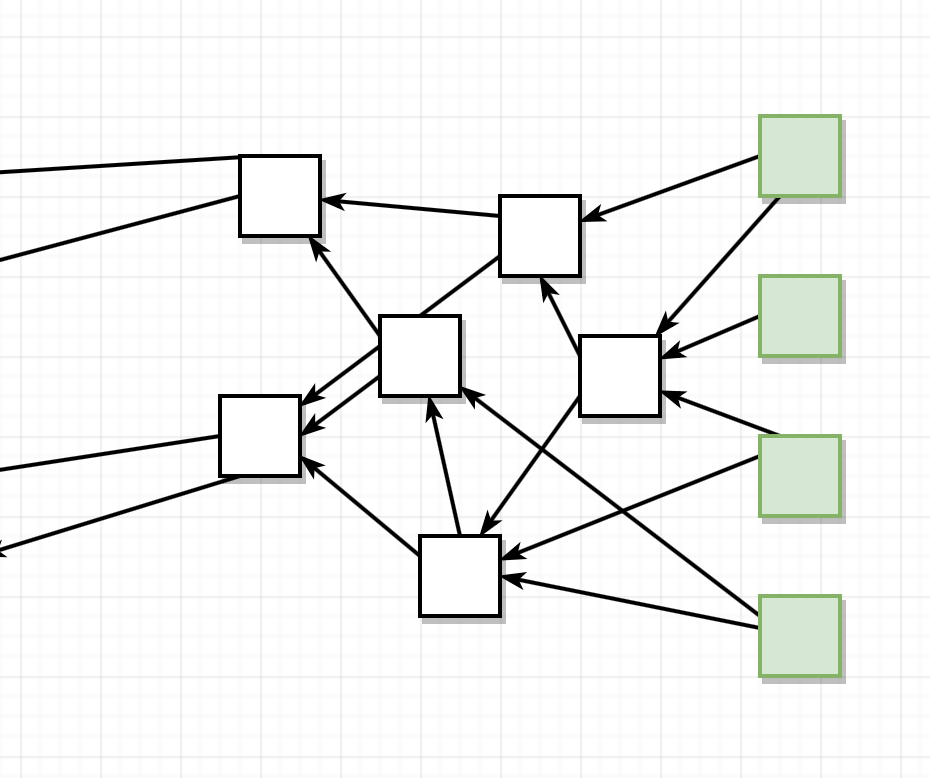
\includegraphics{tangle.png}
%%%%%%%%%%%%%%%%%%%%%%%%%%%%%%%%%%%%%%%%%%%%%%%%%%%%%%%%%%%%%%%%%%%%%%%%
\subsection{Stellar}
%%%%%%%%%%%%%%%%%%%%%%%%%%%%%%%%%%%%%%%%%%%%%%%%%%%%%%%%%%%%%%%%%%%%%%%%

%%%%%%%%%%%%%%%%%%%%%%%%%%%%%%%%%%%%%%%%%%%%%%%%%%%%%%%%%%%%%%%%%%%%%%%%
\subsection{Cardano}
%%%%%%%%%%%%%%%%%%%%%%%%%%%%%%%%%%%%%%%%%%%%%%%%%%%%%%%%%%%%%%%%%%%%%%%%

%%%%%%%%%%%%%%%%%%%%%%%%%%%%%%%%%%%%%%%%%%%%%%%%%%%%%%%%%%%%%%%%%%%%%%%%
\subsection{Neo}
%%%%%%%%%%%%%%%%%%%%%%%%%%%%%%%%%%%%%%%%%%%%%%%%%%%%%%%%%%%%%%%%%%%%%%%%
Originally branded AntShares, NEO was first released in February of 2014. Its stated goal is "to achieve a smart economy with a distributed network"(NEO WHITE PAPER). This smart economy would be constructed on digitized physical assets exchanged through smart contracts. Additionally, NEO offers secure digital identities in accordance with the Public Key Infrastructure X.509 standard. While providing anonymity, NEO therefore offers a viable service for entities who’s actions must comply with financial regulations. It supports a wide range of common programming languages making it accessible to existing industry professionals and decreasing the resources required for retraining staff. Similarly to Ethereum, NEO supports the development of decentralized applications (dapps). It employs a delegated Byzantine Fault Tolerance (dBFT)
%%%%%%%%%%%%%%%%%%%%%%%%%%%%%%%%%%%%%%%%%%%%%%%%%%%%%%%%%%%%%%%%%%%%%%%%
\subsection{Hyperledger}
%%%%%%%%%%%%%%%%%%%%%%%%%%%%%%%%%%%%%%%%%%%%%%%%%%%%%%%%%%%%%%%%%%%%%%%%
A private implementation of Ethereum with a pluggable consensus algorithm. Open sourced by the linux foundation.

%%%%%%%%%%%%%%%%%%%%%%%%%%%%%%%%%%%%%%%%%%%%%%%%%%%%%%%%%%%%%%%%%%%%%%%%
\section{Comparing Implementations}
%%%%%%%%%%%%%%%%%%%%%%%%%%%%%%%%%%%%%%%%%%%%%%%%%%%%%%%%%%%%%%%%%%%%%%%%
In the following sections we will look more closely at different implementations of the Blockchain technology. As of this writing there are more than a thousand cryptocurrencies. To get a good overview we will look at different approaches and exclude hardforks/clones, ICOs and cryptocurrencies without a working product.

%%%%%%%%%%%%%%%%%%%%%%%%%%%%%%%%%%%%%%%%%%%%%%%%%%%%%%%%%%%%%%%%%%%%%%%%
\begin{table}
  %\centering
  \begin{tabular}{llllll}
    \toprule
    \textbf{Blockchain} & \textbf{Genesis} & \textbf{Consensus} & \textbf{\# Clients} & \textbf{Replications} & \textbf{Mining/Security} \\
    \midrule
      \texttt{Bitcoin} & 2009 & Proof of Work & 1 & 1234 \\
      \texttt{Ethereum} & 2009 & Proof of Work & 1 & 1234 \\
      \texttt{Iota} & 2009 & Proof of Work & 1 & 1234 \\
      \texttt{Stellar} & 2009 & Proof of Work & 1 & 1234 \\
      \texttt{Cardano} & 2009 & Proof of Work & 1 & 1234 \\
      \texttt{Neo} & 2009 & Proof of Work & 1 & 1234 \\
      \texttt{Hyperledger} & 2009 & Proof of Work & 1 & 1234 \\
    \bottomrule
  \end{tabular}
  \caption{%
    A table comparing different distributed ledger technologies.
  }
  \label{tab:Packages}
\end{table}
%%%%%%%%%%%%%%%%%%%%%%%%%%%%%%%%%%%%%%%%%%%%%%%%%%%%%%%%%%%%%%%%%%%%%%%%


%%%%%%%%%%%%%%%%%%%%%%%%%%%%%%%%%%%%%%%%%%%%%%%%%%%%%%%%%%%%%%%%%%%%%%%%
\section{Choosing an Implementation}
%%%%%%%%%%%%%%%%%%%%%%%%%%%%%%%%%%%%%%%%%%%%%%%%%%%%%%%%%%%%%%%%%%%%%%%%


